\subsection{CNN BackPropagation}
This subsection is form the slides given in the solution of the exercises 10, the reason for putting it there is that I don't think this materials was taught in class and as far as I know it might be on the exam, so...

\begin{parag}{Backpropagation in CNNs}
    In the backward pass, we get the loss gradient with respect to the next layer. However, in CNNs the loss gradient is computed w.r.t. the input and also w.r.t. the filter. This is the reason why we had to create the function $g_K, g_X$ in the exercises.
\end{parag}
\begin{parag}{Convolution Backprop with single Stride}
    To understand the computation of loss gradient w.r.t input, let us use the following example: 
	\begin{align*} 
		X = \begin{pmatrix} X_{11} & X_{12} & X_{13} \\ X_{21} & X_{22} & X_{23} \\ X_{31} & X_{32} & X_{33} \end{pmatrix} 
	\end{align*}
	And the kernel, Filter 
	\begin{align*} 
		F = \begin{pmatrix} F_{11} & F_{12} \\ F_{21} & F_{22} \end{pmatrix} 
	\end{align*}
	Where we have a horizontal and vertical stride of $1$.\\
	$ $\\
	In the forward pass, the convolution between the input $X$ and the filter $F$ gives us the output O, which can be represented as 
	\begin{align*} 
		\begin{pmatrix} O_{11} & O_{12} \\ O_{21} & O_{22} \end{pmatrix} = \text{Conv}\left(\begin{pmatrix} X_{11} & X_{12} & X_{13} \\ X_{21} & X_{22} & X_{23} \\ X_{31} & X_{32} & X_{33} \end{pmatrix}, \begin{pmatrix} F_{11} & F_{12} \\ F_{21} & F_{22} \end{pmatrix}\right)
	\end{align*}
	Then for instance if we were to compute $O_{11}$ this would be by using  the following
\end{parag}

\begin{center}
	\begin{tikzpicture}[
		scale=0.5,
  cell/.style={
    draw, minimum size=1.1cm, font=\small,
    inner sep=2pt, align=center
  },
  every node/.style={font=\small}
]

%% ── Input matrix X (3×3) ──────────────────────────────────────────────────
\matrix (X) [
  matrix of nodes,
  nodes={cell},
  row sep=-\pgflinewidth,
  column sep=-\pgflinewidth,
  nodes in empty cells
] {
  $X_{11}$ & $X_{12}$ & $X_{13}$ \\
  $X_{21}$ & $X_{22}$ & $X_{23}$ \\
  $X_{31}$ & $X_{32}$ & $X_{33}$ \\
};

% Red border on top-left 2×2 submatrix
\draw[inputred, line width=1.8pt]
  (X-1-1.north west) rectangle (X-2-2.south east);

% Yellow fill on highlighted 2×2 cells
\foreach \r in {1,2} {
  \foreach \c in {1,2} {
    \fill[inputyellow, opacity=0.45]
      (X-\r-\c.north west) rectangle (X-\r-\c.south east);
  }
}

% Redraw cell borders on top of fill
\matrix (X) [
  matrix of nodes,
  nodes={cell},
  row sep=-\pgflinewidth,
  column sep=-\pgflinewidth,
  nodes in empty cells,
  at=(X.center)
] {
  $X_{11}$ & $X_{12}$ & $X_{13}$ \\
  $X_{21}$ & $X_{22}$ & $X_{23}$ \\
  $X_{31}$ & $X_{32}$ & $X_{33}$ \\
};

% Red border redrawn on top
\draw[inputred, line width=1.8pt]
  (X-1-1.north west) rectangle (X-2-2.south east);

% Label below
\node[below=0.3cm of X, font=\small\bfseries] {Input \textbf{X}};

%% ── Convolution symbol ────────────────────────────────────────────────────
\node[right=0.6cm of X, font=\Large] (otimes) {$\otimes$};
\draw[black, line width=0.8pt] 
  ([xshift=-0.35cm, yshift=0.35cm]otimes.center) rectangle
  ([xshift= 0.35cm, yshift=-0.35cm]otimes.center);

%% ── Filter F (2×2) ────────────────────────────────────────────────────────
\matrix (F) [
  matrix of nodes,
  nodes={cell, filterblue},
  row sep=-\pgflinewidth,
  column sep=-\pgflinewidth,
  nodes in empty cells,
  right=0.3cm of otimes,
  yshift=0cm      % vertically centre under ⊗
] {
  $F_{11}$ & $F_{12}$ \\
  $F_{21}$ & $F_{22}$ \\
};

% Label below
\node[below=0.3cm of F, font=\small\bfseries] {Filter \textbf{F}};
\node[right=0.75cm of F, ] {$\implies$};

%% ── Output matrix (3×3) ───────────────────────────────────────────────────
\matrix (R) [
  matrix of nodes,
  nodes={cell, minimum size=1.5cm},
  row sep=-\pgflinewidth,
  column sep=-\pgflinewidth,
  nodes in empty cells,
  right=2.0cm of F,
  yshift=0cm
] {
  $X_{11}F_{11}$ & $X_{12}F_{12}$ & |[resultgray]| $X_{13}$ \\
  $X_{21}F_{21}$ & $X_{22}F_{22}$ & |[resultgray]| $X_{23}$ \\
  |[resultgray]| $X_{31}$ & |[resultgray]| $X_{32}$ & |[resultgray]| $X_{33}$ \\
};

\end{tikzpicture}
\end{center}

Which gives us 

\begin{align*} 
	O_{11} =  X_{11} F_{11} + X_{12} F_{12} + X_{21} F_{21} + X_{22} F_{22}
\end{align*}


\begin{parag}{Loss gradient}
    Now we want to calculate the gradients w.r.t. the input $X$ and filter $F$.\\
\begin{center}
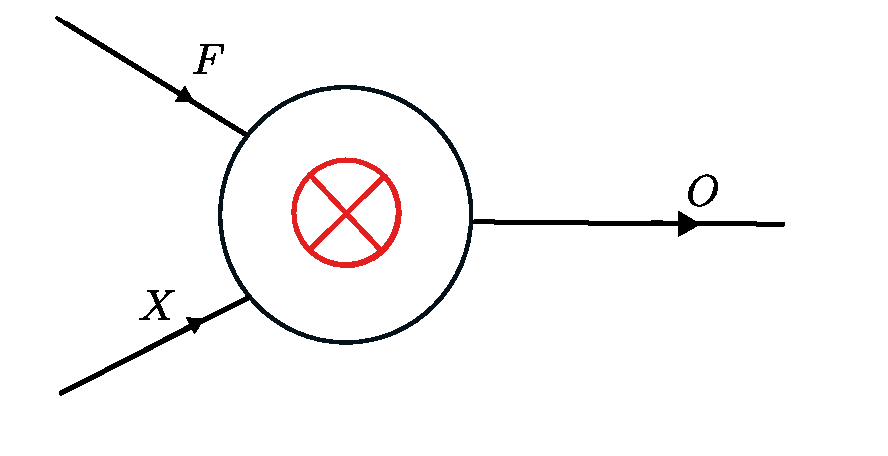
\includegraphics[width=0.4\textwidth]{figure/2026-05-03.pdf}
\end{center}
	$ $\\
	To do so we can use the chain rule to obtain the gradient w.r.t. the filter 
	\begin{align*} 
		\frac{\partial L}{\partial F} = \frac{\partial L}{\partial O}  \frac{\partial O}{\partial F} 
	\end{align*}
	And for every element of $F$:
	\begin{align*} 
		\frac{\partial L}{\partial F_i}  =  \sum_{k= 1}^{M}\frac{\partial L}{\partial O_k}   \frac{\partial O_k}{\partial F_i} 
	\end{align*}

\end{parag}


By replacing the local gradient of the filter i.e., $\frac{\partial O_i}{\partial F_i} $ we get 
\begin{align*} 
	\begin{pmatrix} \frac{\partial L}{\partial F_{11}}  &  \frac{\partial L}{\partial F_{12}} \\  \frac{\partial L}{\partial F_{21}} &  \frac{\partial L}{\partial F_{22}} \end{pmatrix} =  \text{Conv} \left(\begin{pmatrix} X_{11} & X_{12} & X_{13} \\ X_{21} & X_{22} & X_{23} \\ X_{31} & X_{32} & X_{33} \end{pmatrix}, \begin{pmatrix} \frac{\partial L}{\partial O_{11}}  &\frac{\partial L}{\partial O_{12}}  \\\frac{\partial L}{\partial O_{21}}  & \frac{\partial L}{\partial O_{22}} \end{pmatrix} \right)
\end{align*}

If we closely look at it, this represents an operation that we are quit familiar with. We can represent it as a convolution operation between input $X$ and loss gradient $\frac{\partial L}{\partial O} $ as shown here 
\begin{align*} 
	\frac{\partial L}{\partial X_i}  =  \sum_{k= 1}^{M} \frac{\partial L}{\partial O_k}  \frac{\partial O_k}{\partial X_i} 
\end{align*}

First let us rotate the Filter $F$ by 180 degrees. This is done by flipping it first vertically and then horizontally 
\begin{align*} 
	\begin{pmatrix} F_{11} & F_{12} \\ F_{21} & F_{22} \end{pmatrix}  \to \begin{pmatrix} F_{12} & F_{11} \\ F_{22} & F_{21} \end{pmatrix}  \to \begin{pmatrix} F_{22} & F_{21} \\ F_{12} & F_{11} \end{pmatrix} 
\end{align*}
Now we can see that the loss gradient w.r.t. the input $\frac{\partial L}{\partial X} $ is given as a full convolution between the filter (rotated filter) and Loss gradient $\frac{\partial L}{\partial O} $. It is important here to mention the \important{full}.\\
$ $\\
If we were to take the example with the $3 \times 3$ input matrices recall that for each $X_{ij}$ the derivative is given as: 

\begin{align*} 
	\dLdX{1}{1} &= \dLdO{1}{1} F_{11}\\
	\dLdX{1}{2} &= \dLdO{1}{1} F_{12} \;+\; \dLdO{1}{2} F_{11}\\
	\dLdX{1}{3} &= \dLdO{1}{2} F_{12}\\
	\dLdX{2}{1} &= \dLdO{1}{1} F_{21} \;+\; \dLdO{2}{1} F_{11}\\
	\dLdX{2}{2} &= \dLdO{1}{1} F_{22} \;+\; \dLdO{1}{2} F_{21}\;+\; \dLdO{2}{1} F_{12} \;+\; \dLdO{2}{2} F_{11}\\
	\dLdX{2}{3} &= \dLdO{1}{2} F_{22} \;+\; \dLdO{2}{2} F_{12}\\
	\dLdX{3}{1} &= \dLdO{2}{1} F_{21}\\
	\dLdX{3}{2} &= \dLdO{2}{1} F_{22} \;+\; \dLdO{2}{2} F_{21}\\
	\dLdX{3}{3} &= \dLdO{2}{2} F_{22}
\end{align*}
Using that, We can see that 
\begin{align*} 
	\frac{\partial L}{\partial X}  =  \text{Full Conv}\left(\begin{pmatrix} F_{22} & F_{21} \\ F_{12} & F_{11} \end{pmatrix}, \begin{pmatrix} \frac{\partial L}{\partial O_{11}}  & \frac{\partial L}{\partial O_{12}}  \\ \frac{\partial L}{\partial O_{21}}  & \frac{\partial L}{\partial O_{22}}  \end{pmatrix} \right)
\end{align*}
\begin{parag}{Takeaway}
    What is important here is that both forward pass and the Backpropagation of a convolutional layer are \important{convolutions}
	\begin{align*} 
		\frac{\partial L}{\partial F}  = \text{Conv} \left(X, \frac{\partial L}{\partial O} \right)\\
		\frac{\partial L}{\partial X}  \text{Full Conv} \left(\text{180}^{\circ}F, \frac{\partial L}{\partial O} \right)
	\end{align*}

\end{parag}


\begin{parag}{Stride $> 1$}
	Okay this is nice, but now what happen when $s > 1$? For instance let us have a input matrix with only 1 channel with height and width 5. The kernel is a $3 \times 3$ of size with both vertical and horizontal stride of $2$. The output of that convolution would be a $2 \times 2$ $Y$ 
	\begin{align*} 
		Y = \begin{pmatrix} y_{00} & y_{01} \\ y_{10} & y_{11} \end{pmatrix} 
	\end{align*}
\end{parag}
\begin{parag}{Backward Pass}
    We have already seen how the forward pass would look like, so let us go directly into the backward pass. The assumption we will have is that we have the loss gradient w.r.t. the output pixels. meaning we have 
	\begin{align*} 
		\begin{pmatrix} \frac{\partial L}{\partial y_{00}}  & \frac{\partial L}{\partial y_{01}}  \\ \frac{\partial L}{\partial y_{10}}  & \frac{\partial L}{\partial y_{11}}  \end{pmatrix} 
	\end{align*}
	and we want to do into the loss gradient w.r.t. the input (of size $5 \times 5$).\\
	$ $\\
	As each input contributes to one or more outputs. The total gradient of the loss w.r.t. each input pixel is computed using 
	\begin{align*} 
		\frac{\partial L}{\partial x_mn} = \sum_{ij} \frac{\partial L}{\partial y_{ij}} \frac{\partial y_{ij}}{\partial x_{mn}} 
	\end{align*}
	The gradient computation is done using the chain rule where $i$ and $j$ represent the position of a single output pixel.
	\begin{subparag}{Example}
	    Let us consider the input $x_{00}$, this input contributed to the output $y_{00}$. On the other hand the input $x_{01}$ contributed to $y_{00}$ therefore, the loss gradientw.r.t. $x_{01}$ is computed as 

		\begin{align*} 
			\frac{\partial L}{\partial x_{01}} = \frac{\partial L}{\partial y_{00}} f_{01}
		\end{align*}
		Now the input $x_{02}$ contributed to the output $y_{00}$ and $y_{01}$ so the loss gradient w.r.t. $x_{02}$ is computed as shown 
		\begin{align*} 
			\frac{\partial L}{\partial x_{02}} = \frac{\partial L}{\partial y_{00}} f_{02} + \frac{\partial L}{\partial y_{01}}  f_{00}
		\end{align*}
		To visualize the pattern more clearly, we pad the gradient tensor with zeros at the top and bottom as well as to the left and right. The number of zeros padded on either side is equal to the stride (horizontal and vertical). We also dilate the output gradient pixels with the stride (vertically and horizontally)
	\end{subparag}
	And as in the previous example we rotate the filter vertically and horizontally and using those two tricks, convolving with a stride greater than $1$ is the same as convolving with a stride of 1 and '\textit{dropping}' out every rows, and every columns that doesn't count in the stride.
\end{parag}




